\section{Ziel}
Ziel des folgenden Experiments ist, mithilfe der Dopplersonographie die Strömung einer für diese Anwendung blutähnlichen Flüssigkeit (Suspension aus Wasser, Glycerin und Glaskügelchen) näher zu untersuchen.

\section{Theorie}
\label{sec:theorie}
\subsection{Schall}
Schall, also allgemein die Ausbreitung von Druckwellen innerhalb von Medien, kann anhand seiner Freqeunz in zwei Bereiche unterteilt werden:
\begin{enumerate}
  \item <\SI{16}{\Hz}: Infraschall
  \item \SI{20}{\kilo\Hz} -- \SI{1}{\giga\Hz}: Ultraschall
\end{enumerate}
Der für Menschen hörbare Schall befindet sich im Bereich von $\SI{16}{\Hz}$ -- $\SI{20}{\kilo\Hz}$. In diesem Experiment wird Ultraschall benutzt, um die Flüssigkeitsströmung zu untersuchen.

\subsection{Piezoelektrischer Effekt}
Es stellt sich die Frage, wie Ultraschall erzeugt werden kann. Eine Möglichkeit ist die Nutzung des reziproken piezoelektrischen Effekts.
Im Allgemeinen wird unter dem piezoelektrischen Effekt verstanden, dass durch Verformung eines Kristalls eine Spannung auftritt. Der reziproke piezoelektrische Effekt bezeichnet den Vorgang, dass es durch eine Spannung (Kristall im elektrischen Wechselfeld) zu Verformungen kommt.

In der konkreten Anwendung befindet sich ein Kristall mit einer polaren Achse in Feldrichtung in einem elektrischen Wechselfeld. Der Kristall beginnt zu schwingen und sendet dabei Ultraschallwellen aus. Wird ein piezoelektrischer Kristall als Schallempfänger verwendet, wird dieser von auftreffenden Schallwellen zum Schwingen angeregt, die auftretende Spannung kann gemessen werden.

\subsection{Doppler-Effekt}
Bewegen sich Schallquelle und der Empfänger relativ zueinandern, tritt eine Frequenzänderung auf. Dies wird als Doppler-Effekt bezeichnet.
Zunächst wird der Fall mit ruhendem Empfänger und sich bewegender Quelle betrachtet. Wenn sich die Quelle in Richtung des Empfängers bewegt, wird die Frequenz $f_0$ zu $f_\mathrm{kl}$ erhöht und es gilt folgender Zusammenhang:
\begin{equation}
  f_\mathrm{kl} = \frac{f_0}{1-\frac{v}{c}}
\end{equation}
Dabei ist $v$ die Geschwindigkeit der Quelle und $c$ die Schallgeschwindigkeit.
Bewegt sich der Sender vom Empfänger weg, fällt die Frequenz auf $f_\mathrm{gr}$.
\begin{equation}
  f_\mathrm{gr} = \frac{f_0}{1+\frac{v}{c}}
\end{equation}
Im Folgenden bewegt sich der Empfänger und der Sender befindet sich in Ruhe. Wenn sich der Empfänger der Quelle nähert, verschiebt sich $f_0$ zu einer größeren Frequenz $f_\mathrm{h}$
\begin{equation}
  f_\mathrm{h} = f_0\left(1+\frac{v}{c}\right)
\end{equation}
mit  $v$ als Geschwindigkeit des Empfängers und $c$ als Schallgeschwindigkeit.
Die Frequenz sinkt auf eine kleinere Frequenz $f_\mathrm{n}$, wenn die Entfernung zwischen Sender und Empfänger durch die Bewegung des Empfängers steigt.
\begin{equation}
  f_\mathrm{n} =f_0\left(1-\frac{v}{c}\right)
\end{equation}

Mit Hilfe des beschriebenen Doppler-Effekts kann die Geschwindigkeit von Blutströmungen bestimmt werden. Beim Auftreffen auf sich bewegende Blutkörper wird die Frequenz $f_0$ der Ultraschallwelle wie folgt verschoben:
\begin{equation}
  \Delta f = f_0 \frac{v}{c}(\cos\alpha + \cos\beta)
\end{equation}
mit $\alpha$ als Winkel zwischen der Wellennormalen und der einlaufenden Welle und $\beta$ als Winkel zwischen der Wellennormalen und der auslaufenden Welle. Da beim Impuls-Echo-Verfahren $\alpha = \beta$ (siehe Abbildung \ref{fig:1}) gilt, folgt:
\begin{equation}
  \label{eqn:delta_f}
  \Delta f = 2\,f_0\frac{v}{c}\cos\alpha
\end{equation}

\begin{figure}
  \centering
  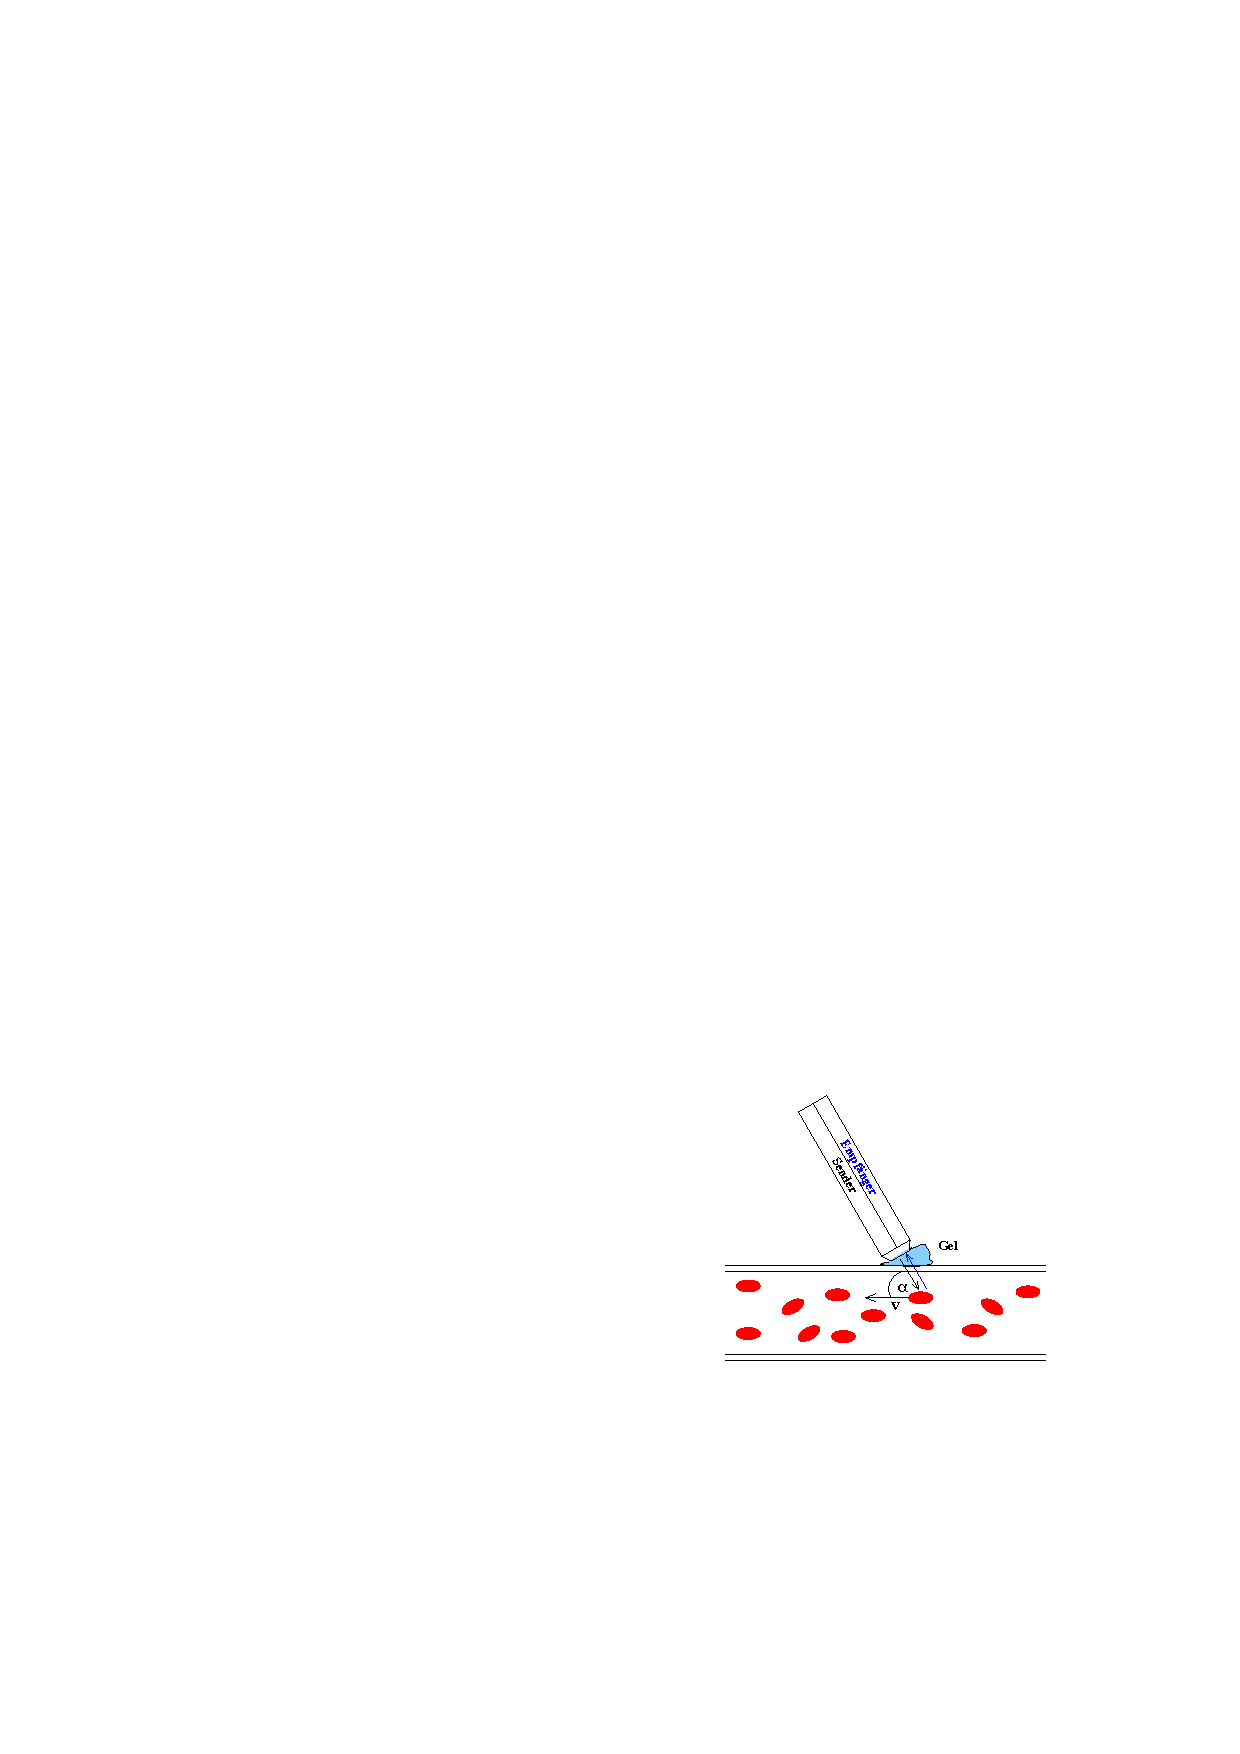
\includegraphics[scale=0.8]{content/1.pdf}
\caption{Messung der Geschwindigkeit von Blutströmungen mittels Impuls-Echo-Verfahren\cite{anleitungUS3}.}
  \label{fig:1}
\end{figure}
